Come accennato in precedenza, le simulazioni fluidodinamiche risultano
particolarmente onerose da un punto di vista computazionale, sia in termini di
hardware che di software. Da un punto di vista hardware la numerosa quantità di
particelle, celle, volumi e mesh ad alta risoluzione possono gravare sulla memoria primaria del
calcolatore. D'altro canto la quantità di questi elementi inficia negativamente
anche le prestazioni del processore che viene oberato dei calcoli matematici
descritti nel capitolo \ref{cap:capitoli/capitolo2/capitolo2}. \newline
Da un punto di vista software invece le difficoltà si celano nel tentativo di
ottimizzazione dell'utilizzo delle risorse computazionali. Proprio per questo motivo
le scelte di linguaggio, compilatore e librerie risultano critiche da un punto di vista
prestazionale.


\section{Linguaggi Utilizzati}
Inizialmente il simulatore venne abbozzato utilizzando Python come linguaggio e
Fenics \cite{AlnaesBlechta2015a} come risolutore di equazioni differenziali alle derivate
parziali e LEoPart \cite{maljaars2020} per simulare l'avvezione delle particelle.
Per quanto sia apprezzabile la facilità d'uso di Python si è rivelato in poco tempo un
linguaggio poco adatto al nostro caso d'uso (la spiegazione nella sottosezione dedicata),
si è optato quindi per utilizzare un linguaggio più performante come C++ e che, soprattutto,
è molto più usato per simulazioni di questo tipo. La popolarità di C++ nel campo delle simulazioni, in generale laddove sono necessarie performance
(videogiochi 3D, High Performance Computing, sistemi embedded, industria cinematografica),
rende anche più facile reperire materiale, librerie e pubblicazioni riguardo l'argomento.
    \subsection{Python versione 3.6}\label{python}
    Python è un linguaggio di programmazione ad alto livello, orientato a oggetti, molto utilizzato
    in ambito matematico, fisico e scientifico ideato da Guido van Rossum\cite{10.5555/1593511}. L'obiettivo principale di Python
    è dare la possibilità agli utenti di realizzare complesse applicazioni in modo semplice e veloce.
    La sintassi di Python obiettivamente risulta semplice combinata con la possibilità di utilizzare
    il paradigma di programmazione orientata agli oggetti lo rendono estremamente leggibile e manutenibile.
    Il fatto che Python sia un linguaggio interpretato rende anche veloce il ciclo di sviluppo (modifica, test, rilascio).
    La possibilità di estendere Python con librerie C, C++ è ciò che lo rende utilizzabile anche per computazioni
    complesse. L'estendibilità è un punto di forza di Python, esistono infatti una grande varietà
    di librerie di terze parti per soddisfare pressoché qualsiasi caso d'uso.
    Python viene sviluppato con licenza OpenSource.
    \begin{figure}[H]
        \centering
        
\includegraphics[width=\linewidth]{figure/python.png}
        \caption{Logo Python}
    \end{figure}

    \subsection{C++}
    C++ è un linguaggio di programmazione compilato, di livello più basso rispetto a Python, inventato da Bjarne
    Stroustrop come successore del linguaggio C e, dal 1998, standardizzato da WG21 \cite{ISO:1998:IIP}. Nel corso
    degli anni sono state rilasciate diverse versioni con migliorie e nuove funzionalità, tra le più recenti ci sono:
    C++17 \cite{Cpp17} e C++20 \cite{N4817}. Il linguaggio si presta a diversi paradigmi di programmazione tra cui:
    \begin{itemize}
        \item Orientata a oggetti
        \item Funzionale
        \item Procedurale
    \end{itemize}
    Alcune caratteristiche rilevanti del linguaggio:
    \begin{itemize}
        \item Tipizzazione forte: assicura che eventuali errori di compilazione siano rilevati subito
        \item Insicurezza di esecuzione: gli errori non sono completamente gestiti e si
        ha accesso diretto alla memoria dei processi
        \item Multi-piattaforma
        \item Gestione della memoria manuale
    \end{itemize}

    Come anticipato C++ fa affidamento a un compilatore per generare eseguibili, il processo di
    compilazione può essere suddiviso in tre principali passi:

    \paragraph{Preprocessamento:}
    Il preprocessore è responsabile di gestire tutte le direttive di preprocessamento tra cui:
    \begin{itemize}
        \item \texttt{\#include}
        Per referenziare librerie esterne o interne all'interno di un file.
        \item \texttt{\#define MACRO=1}
        Per definire un simbolo, o MACRO, che verrà poi sostituito all'interno del codice.
        \item \texttt{\#if \#ifdef \#ifndef}
        Per abilitare o disabilitare porzioni di codice.
    \end{itemize}
    Dopo aver applicato le corrette sostituzioni alle varie direttive il preprocessore produce un artefatto
    consumabile dal compilatore.\par

    \paragraph{Compilazione:}\label{c++}
    Gli artefatti che arrivano dal preprocessore vengono trattati dal compilatore come puro codice sorgente
    C++, che li interpreta e li converte in codice macchina producendo diversi file binari (uno per file
    di codice). Questa fase è responsabile per la generazione di librerie statiche, utili per il riuso del codice.
    In questa fase vengono sollevati gli errori di compilazione.\par

    \paragraph{Linking:}
    Il "linker" è il componente che produce eseguibili, librerie condivise (o dinamiche) collegando i diversi
    artefatti prodotti dal compilatore. Il processo prevede la referenziazione di tutti i simboli lasciati indefiniti
    dal compilatore con gli oggetti corretti, sia che essi siano in librerie condivise o in altri file.\par
    \noindent
    \newline
    La grande varietà di compilatori disponibili rende C++ portabile e multi-piattaforma, inoltre essendo
    un'evoluzione di C è anche compatibile con codice C e le librerie sviluppate per esso.

    \subsubsection{Template Metaprogramming}\label{template}
    Deal.II \ref{dealii} fa largo uso di un sistema di metaprogrammazione presente in C++. Il sistema
    permette di eseguire svariate operazioni in fase di compilazione che elaborano il codice sorgente.
    Prevalentemente le operazioni vengono svolte sui tipi utilizzati all'interno del programma.
    In C++ è presente un rigoroso controllo statico dei tipi che rende necessario definire a priori
    il tipo delle variabili che vengono usate come argomenti per funzioni o membri di classe. Questo fattore
    va contro uno dei principi fondamentali della programmazione, il riutilizzo del codice. Per ovviare a questo vincolo
    C++ offre una parola chiave che viene usata per indicare porzioni di codice generiche, \textit{template}.
    Esempio di funzione che somma due tipi generici:
    \begin{verbatim}
        template <typename T>
        T somma_tra_generics(T a, T b) {
            return a+b;
        };
        int main() {
            int i1 = 1;
            int i2 = 2;
            int sum =  somma_tra_generics(i1,i2);
            std::cout << sum << std::endl;
            return 0;
        }
    \end{verbatim}

    In fase di pre-compilazione ogni funzione, o classe, che viene preceduta dalla parola chiave \textit{template}
    viene processata generando a sua volta nuove funzioni e nuovi classi per ogni tipo di variabile con cui essa viene convocata. Al contrario di linguaggi come Java, non c'è nessun tipo di
    overhead o virtual tables. Java per esempio riesce a implementare i tipi generici utilizzando delle virtual tables dove il tipo generico viene trattato come oggetto base per poi essere
    risolto a runtime. Nell'esempio precedente viene creata una sola istanza di template per il tipo \textit{int}.
    Il sistema di \textit{template} in C++ è turing-completo, nel senso che può eseguire
    una serie di istruzioni condizionali e ricorsive di complessità arbitraria.
    Avvalersi della metaprogrammazione attraverso template rende la creazione di
    librerie di basso livello più facile e consente di crearle efficienti e flessibili.

    \subsubsection{Prestazioni}
    C++ è considerato un linguaggio molto performante e efficiente, parte delle ragioni sono descritte di seguito.

    \paragraph{Strutture dati ottimizzate}
    Le strutture dati che offre C++, e le librerie standard, non hanno nessun tipo di overhead di memoria,
    quindi per costruzione occupano il minimo indispensabile della memoria che serve per veicolare
    l'informazione contenuta. Una struttura dati più piccola rappresenta una gestione migliore della cache e
    della memoria principale.
    \par

    \paragraph{Compilatori ottimizzati}
    C++ è un linguaggio maturo che vanta una grande varietà di compilatori che nel tempo sono stati estremamente ottimizzati
    per tradurre codice sorgente in codice macchina in maniera efficiente.
    \par

    \paragraph{Puntatori diretti}
    Come in C, C++ ha la possibilità di referenziare zone di memoria con dei puntatori in modo diretto.
    Questa possibilità rende il codice potenzialmente insicuro, ma allo stesso tempo da modo allo sviluppatore
    di accedere alle risorse velocemente. Recentemente l'avvento degli Smart Pointers (puntatori intelligenti)
    ha reso l'utilizzo dei puntatori molto più sicuro.
    \par



    \section{Librerie e Framework}

    Per riuscire a simulare casi d'uso complicati come quello descritto in questa tesi
    sarebbe impensabile sviluppare ogni singolo risolutore di PDE
    (\ref{PDE}), convertitore di mesh o sistema di gestione
    thread. Per ovviare a questo problema ci avvaliamo di alcune librerie Open-Source che
    altri sviluppatori, matematici, fisici e ingegneri hanno realizzato per risolvere problemi
    simili. Di seguito alcune librerie che hanno influenzato lo sviluppo della soluzione
    proposta.

    \subsection{Intel TBB}\label{tbb}
    Intel TBB, acronimo per Threading Building Blocks, è una libreria C++ basata su template (\ref*{template})
    che facilita l'implementazione di paradigmi di programmazione parallela \cite{KukanovAlexey2007TFfS}.
    Un programma che utilizza TBB riesce a creare diversi grafi di task dipendenti fra loro, a
    organizzarli e sincronizzarli in maniera efficiente e, a task completato, distruggerli. TBB fa uso
    di una tecnica di bilanciamento di carico parallelo chiamata "work stealing" (letteralmente, furto del lavoro),
    che bilancia i task che sono in attesa in maniera dinamica verso core scarichi. Il vantaggio di TBB
    è che fa tutte queste ottimizzazioni in maniera automatica offrendo interfacce di alto livello che rendono
    semplice l'implementazione. TBB è una libreria che gestisce carichi di lavoro paralleli, ma non garantisce
    l'esenzione dalle cosidette \textit{corse critiche (race conditions)}.
    TBB offre diversi algoritmi di base:

    \begin{itemize}
        \item \texttt{parallel\_for}
        \item \texttt{parallel\_reduce}
        \item \texttt{parallel\_scan}
    \end{itemize}

    e avanzati:

    \begin{itemize}
        \item \texttt{parallel\_while}
        \item \texttt{parallel\_do}
        \item \texttt{parallel\_pipeline}
        \item \texttt{parallel\_sort}
    \end{itemize}

    Oltre agli algoritmi sono disponibili diverse strutture e modalità di allocazione dati, operazioni atomiche
    e funzioni di timing e task scheduling. Vediamo un esempio di come implementare un semplice \texttt{parallel\_for} sfruttando TBB.

    Come prima cosa includiamo le librerie di cui abbiamo bisogno:
    \begin{verbatim}
#include "tbb/blocked_range.h" //Range divisibile ricorsivamente
#include "tbb/parallel_for.h" //Algoritmo
#include "tbb/task_scheduler_init.h" // Scheduler di task
#include <iostream>
#include <vector>
    \end{verbatim}
    Dichiariamo la struttura che incapsula il nostro task:
    \begin{verbatim}
struct task {
    task(size_t n): _n(n)    {}
    void operator()() {
        //Istruzioni arbitrarie che vengono eseguite in parallelo
        for (int i=0;i<1000000;++i) {}
        std::cerr << "[" << _n << "]";
    }
    size_t _n;
};
    \end{verbatim}
    La struttura che esegue i task accetta un vettore di task e ha una funzione che splitta i task e li esegue parallelamente:
    \begin{verbatim}
struct executor
{

    executor(std::vector<task>& t)
    :_tasks(t)
    {}
    executor(executor& e,tbb::split)
    :_tasks(e._tasks)
    {}

    void operator()(const tbb::blocked_range<size_t>& r) const {
    for (size_t i=r.begin();i!=r.end();++i)
        _tasks[i]();
    }

    std::vector<task>& _tasks;
};
    \end{verbatim}
    \begin{verbatim}
int main(int,char**) {
  // Vengono automaticamente inizializzati i threads
  tbb::task_scheduler_init init;

  // Creiamo dei task e li inseriamo in un vettore
  std::vector<mytask> tasks;
  for (int i=0;i<1000;++i)
    tasks.push_back(mytask(i));

  // Creiamo l'executor dei task e invochiamo l'algoritmo TBB
  executor exec(tasks);
  tbb::parallel_for(tbb::blocked_range<size_t>(0,tasks.size()),exec);
  std::cerr << std::endl;

  return 0;
}
    \end{verbatim}

    \subsection{MPI}
    MPI, acronimo di Message Passing Interface, è un protocollo di comunicazione per calcolatori \cite{10.5555/898758}. È ormai
    uno standard di comunicazione usato espressamente per lo scambio di informazioni in calcoli paralleli.
    MPI è una specifica, non una libreria, di conseguenza esistono diverse librerie che la implementano.
    L'obiettivo della specifica è quello di fornire un paradigma di programmazione parallela che sia pratico,
    efficiente e portabile. Lo standard non specifica come eseguire i programmi, piuttosto ogni implementazione
    fornisce diversi strumenti per compilare ed eseguire programmi MPI. In fase di esecuzione ogni programma
    implementato con MPI ha a disposizione due funzioni per conoscere il numero di processi che partecipano
    all'esecuzione parallela e il proprio identificativo di processo. Lo standard inoltre definisce come
    le informazioni debbano essere comunicate ai vari processi, incapsulando l'informazione in un messaggio
    che contiene il buffer di dati, il numero di elementi da inviare e il tipo di dato. Il messaggio viene
    inviato indicando un destinatario, individuato attraverso tag, rank (identificativo processo) e
    comunicatore (gruppo di processi). Esiste un comunicatore di default a cui appartengono tutti i processi
    chiamato MPI\_COMM\_WORLD. MPI può operare sia in maniera asincrona (sia bloccanti che non) che in sincrona, a discrezione dell'utente.
    Un protocollo di comunicazione che permette di scalare su più processori o calcolatori una simulazione CFD
    è di vitale importanza poiché, come accennato in precedenza, la grande quantità di calcoli richiesti
    rende i tempi di esecuzione molto lunghi anche per piccole simulazioni con pochi elementi.
        \subsubsection{OpenMPI}
        OpenMPI è una popolare implementazione del protocollo MPI, sviluppata e manutenuta da un consorzio
        di accademici, ricercatori e partner. Alcune caratteristiche che rendono OpenMPI un ottima libreria
        che implementa MPI:

        \begin{itemize}
            \item Alto livello di thread-safety e concorrenza
            \item Possibilità di generazione processi in modo dinamico
            \item Tolleranza in caso di errori di rete o processo
            \item Compatibile con una grande varietà di sistemi operativi
            \item Prestazioni elevate su ogni piattaforma supportata
            \item Portabile e estendibile
            \item Sviluppo e supporto dalla community attivo
            \item Licenza open-source
        \end{itemize}

        \begin{figure}[H]
            \centering
            
\includegraphics[width=0.25\textwidth]{figure/openmpi.png}
            \caption{Logo OpenMPI}
        \end{figure}
        Di seguito un piccolo esempio di come utilizzare la libreria di OpenMPI che stampa a schermo il numero di processori di un calcolatore e il loro rango.
        Come prima cosa includiamo le librerie necessarie:
        \begin{verbatim}
#include <mpi.h>
#include <stdio.h>
        \end{verbatim}
        All'interno di una funzione \texttt{int main(int argc, char** argv)} inizializziamo MPI con:
        \begin{verbatim}
MPI_Init(NULL,NULL);
        \end{verbatim}
        Ricaviamo il numero di processi con:
        \begin{verbatim}
int world_size;
MPI_Comm_size(MPI_COMM_WORLD, &world_size);
        \end{verbatim}
        Prendiamo il rank del processo:
        \begin{verbatim}
int world_rank;
MPI_Comm_rank(MPI_COMM_WORLD, &world_rank);
        \end{verbatim}
        Stampiamo e liberiamo le risorse MPI:
        \begin{verbatim}
printf("Processore %d su %d", world_rank,world_size);
MPI_Finalize();
        \end{verbatim}
        Per far si che il programma venga eseguito in parallelo, lo compiliamo normalmente e lo eseguiamo così:
        \begin{verbatim}
mpirun -n NUMERO_PROCESSORI NOME_FILE
        \end{verbatim}
        che stamperà su schermo una riga per ogni numero di processori passato all'istruzione \texttt{mpirun}.
    \subsection{OpenFoam}
    OpenFoam, ovvero Open Field Operation And Manipulation \cite{doi:10.1063/1.168744}, è una libreria C++
    che offre una serie di strumenti per sviluppare software di simulazione.
    OpenFoam è un finalizzatore (chiamato anche Solver) che si basa sulla teoria
    della meccanica dei continui e che include moduli di fluidodinamica computazionale.
    OpenFoam offre strumenti per simulare situazioni derivanti da diversi ambiti fisici.
    Una serie, non esaustiva di strumenti che OpenFoam fornisce:
    \begin{itemize}
        \item Operazioni su tensori e campi
        \item Discretizzazione di equazioni alle derivate parziali
        \item Soluzione di sistemi lineari
        \item Soluzione di equazioni alle derivate ordinarie
        \item Parallelizzazione automatica di operazioni di alto livello
        \item Gestione di mesh dinamiche
    \end{itemize}

    Questi strumenti sono utilizzati per risolvere i seguenti modelli:
    \begin{itemize}
        \item     Modelli reologici
        \item     Modelli termodinamici
        \item     Modelli di turbolenza
        \item     Reazioni chimiche e modelli cinetici
        \item     Tracciamento di particelle lagrangiane
        \item     Modelli di trasferimento di calore per radiazione
        \item     Metodi a singolo e multiplo sistema di riferimento
    \end{itemize}

    Tra i tutti i solver che sono inclusi in OpenFoam ricordiamo:
    \begin{itemize}
        \item Fluidodinamica computazionale
        \item Flussi incomprimibili
        \item Flussi comprimibili
        \item Dinamica dei solidi
        \item Combustione
    \end{itemize}
    OpenFoam offre anche diverse utility per la generazione, la conversione e la manipolazione delle mesh,
    parallelizzazione, pre/post-processing.
    Un punto di forza che contraddistingue OpenFoam è la possibilità che da all'utente di creare Solvers autonomamente.
    Purtroppo OpenFoam, però, presenta diversi tipi di problemi che ne rendono l'utilizzo estremamente difficile.
    In primis la documentazione è molto scarna, soprattutto quando si tratta di lavorare con delle mesh particolarmente complesse. La curva di apprendimento di OpenFoam proprio per questo motivo è estremamente ripida.
    La documentazione pressoché assente spesso implica dei costi nascosti quali: ore di lavoro buttate, corsi di aggiornamento o addestramento e consulenze esterne.
    Quest'ultime sono molto costose proprio per la criticità del settore e impattano l'esperienza open source del prodotto.
    Alcune scelte implementative effettuate da OpenFoam sono obiettivamente considerate in constrasto con le convenzioni di programmazione, soprattutto in ambito C/C++,
    un esempio lampante sono le direttive include all'interno del corpo delle funzioni.
    Infine un ulteriore motivo per cui OpenFoam è stata scartata è l'impossibilità di formulare un problema in cui si accoppia fluido e particelle integrando il campo della temperatura.

    Vediamo un piccolo esempio di programma che interpreta una mesh utilizzando OpenFoam:
    \begin{verbatim}
#include "fvCFD.H"

int main(int argc, char *argv[])
{
    #include "setRootCase.H"

    //Qui creiamo il time system e l'istanza della mesh.
    //notare le direttive di include nel corpo della funzione.
    #include "createTime.H"
    #include "createMesh.H"


    // Iteriamo le celle della mesh e stampiamone a schermo 1 su 20
    for (label cellI = 0; cellI < mesh.C().size(); cellI++)
        if (cellI == 0)
            Info
            << "Cella: "
            << cellI
            << " centrata in: "
            << mesh.C()[cellI]
            << endl;
    Info << endl;

    // Ogni cella è costituita da facce interne o di contrno
    for (label faceI = 0; faceI < mesh.owner().size(); faceI++)
        if (faceI == 0)
            Info
            << "Faccia interna: "
            << faceI
            << " centrata in "
            << mesh.Cf()[faceI]
            << " cella padre " << mesh.owner()[faceI]
            << " cella vicina " << mesh.neighbour()[faceI] << endl;
    Info << endl;

    // Le condizioni al contorno sono accedute
    // attraverso boundaryMesh().
    // OpenFOAM fornisce dei for custom per ridurre il numero
    // di codice da scrivere.
    forAll(mesh.boundaryMesh(), patchI)
        Info 
        << "Patch " 
        << patchI 
        << ": " 
        << mesh.boundary()[patchI].name() << " con "
        << mesh.boundary()[patchI].Cf().size() << " facce. "
        << mesh.boundary()[patchI].start() << endl;
    Info << endl;

    // Le facce adiacenti a dei contorni sono accedute così.
    label patchFaceI(0);
    forAll(mesh.boundaryMesh(), patchI)
        Info << "Patch " 
            << patchI 
            << " ha una faccia " 
            << patchFaceI 
            << " adiacente alla cella "
            << mesh.boundary()[patchI].patch().faceCells()[patchFaceI]
            << ". Normale " << mesh.boundary()[patchI].Sf()[patchFaceI]
            << " superficie " 
            << mag(mesh.boundary()[patchI].Sf()[patchFaceI])
            << endl;
    Info << endl;

    // Si possono iterare anche i singoli 
    // punti o vertici della mesh
    const faceList& fcs = mesh.faces();
    const List<point>& pts = mesh.points();
    const List<point>& cents = mesh.faceCentres();

    forAll(fcs,faceI)
        if (faceI%80==0)
        {
            if (faceI<mesh.Cf().size())
                Info << "Internal face ";
            else
            {
                forAll(mesh.boundary(),patchI)
                    if ((mesh.boundary()[patchI].start()<= faceI) &&
                        (
                            faceI < mesh
                            .boundary()[patchI]
                            .start()+mesh
                            .boundary()[patchI]
                            .Cf()
                            .size())
                        )
                    {
                        Info << "Faccia su Patch " 
                        << patchI 
                        << ", faceI ";
                        break;
                    }
            }

            Info << faceI << " centrata in " << cents[faceI]
                    << " ha " << fcs[faceI].size() << " vertici:";
            forAll(fcs[faceI],vertexI)
                Info << " " << pts[fcs[faceI][vertexI]];
            Info << endl;
        }
    Info << endl;

    return 0;
}
    \end{verbatim}
    \begin{figure}[H]
        \centering
        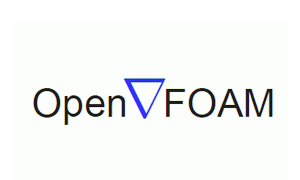
\includegraphics[width=0.4\textwidth]{figure/openfoam.png}
        \caption{Logo OpenFoam}
    \end{figure}

    \subsection{FEniCS Project}\label{fenics}
    FEniCS è una piattaforma open-source il cui scopo è il calcolo di equazioni alle derivate parziali \cite{LoggOlgaardEtAl2012a}.
    FEniCS utilizza un interfaccia di alto livello scritta in Python che facilità l'implementazione a chi non
    ha esperienze pregresse di programmazione. FEniCS fa largo uso di librerie C++ che offrono
    a chi usa questa piattaforma elevate prestazioni. FEniCS è ottimizzata per essere usata su anche su
    cluster di calcolatori molto performanti.
    Nonostante sia una piattaforma molto popolare per la risoluzione PDE (\ref{PDE}) attraverso metodo FEM, l'idea di
    implementare un simulatore di flussi particellari è stata scartata, principalmente per problemi di compatibilità fra diversi sistemi
    , ma non solo. Per quanto sia possibile utilizzare Anaconda \ref*{anaconda} per risolvere le dipendenze dei pacchetti usati da Fenics,
    questo spesso non garantisce il corretto funzionamento su piattaforme uguali. Inoltre nonostante sia una libreria in circolazione
    dal 2005 viene spesso aggiornata deprecando intere librerie di computazione matematica tra una versione e l'altra.
    Oltre a ciò le interfacce fra C++ e Python non sono ancora propriamente separate, il namespacing non è intuitivo,
    la parallelizzazione non sfrutta a pieno le risorse computazionali messe a disposizione e la documentazione è ancora poco dettagliata.
    \begin{figure}[H]
        \centering
        
\includegraphics[width=\linewidth]{figure/fenics.png}
        \caption{Logo Fenics}
    \end{figure}

        \subsubsection{LEoPart}\label{leopart}
        LEoPart (Langrangian-Eulerian on Particles) integra alcune funzionalità riguardanti i flussi
        di particelle in FEniCS \cite{maljaars2020}. L'obiettivo della libreria è quello di occuparsi
        di avvezione e proiezione di particelle in una mesh in modo accurato e conservativo. La libreria è
        stata scartata poiché ha subito diverse modifiche durante lo sviluppo di questo progetto, inoltre
        integrare la simulazione della temperatura del fluido risultava particolarmente complicato.


    \subsection{deal.II}\label{dealii}
    Deal.II, o Differential Equations Analysis Library versione 2 (II), è una libreria che ha come obiettivo la risoluzione
    di equazioni differenziali alle derivate parziali attraverso l'utilizzo del metodo degli elementi finiti \cite{dealII92}.
    È una libreria moderna e open-souce che fornisce un interfaccia semplice capace di sfruttare complessi algoritmi
    e strutture dati per risolvere problemi numerici, il tutto in maniera molto efficiente e performante.
    Questa libreria, alla base di molti strumenti di simulazione moderni, rende il processo di sviluppo rapido
    e sicuro, offrendo una serie di funzionalità ... [aggiungi funzionalità e funzionamento]
    \begin{figure}[H]
        \centering
        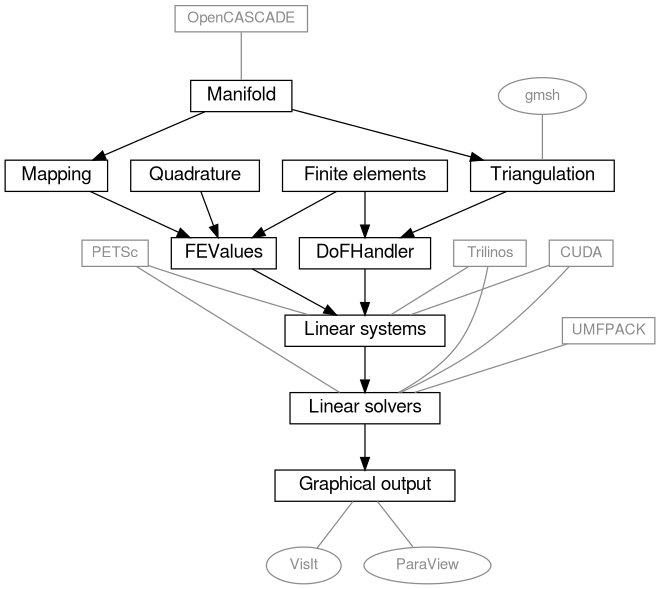
\includegraphics[width=\linewidth]{figure/dealii-detail.png}
        \caption{Architettura deal.II}
    \end{figure}
    \newpage\newpage
    \subsection{Aspect}
    Aspect, acronimo per Advanced Solver for Problems in Earth's ConvecTion \cite{aspectmanual}, è un programma open-source
    sviluppato in C++ che supporta la ricerca simulando diversi tipi di scenari tra cui:
    \begin{itemize}
        \item Convezione del mantello terrestre
        \item Convezione di metalli vicini al nucleo terrestre
        \item Deformazione litosferica
        \item Flussi bifasici
    \end{itemize}
    Aspect ha avuto un impatto importante nello sviluppo di questo progetto, essendo un programma che simula
    problemi di convezione termica ha contribuito in alcune scelte tecniche che discuteremo più avanti.
    Aspect fa largo uso di deal.II per creare e risolvere problemi descritti da equazioni differenziali
    alle derivate parziali attraverso l'uso del metodo degli elementi finiti.

\section{Strumenti di sviluppo}
Per ovviare alle difficoltà che si presentano in fase di sviluppo di progetti con molteplici dipendenze e che si avvalgono
dell'utilizzo di altrettante librerie di terze parti, è altamente consigliato progettare un ambiente di sviluppo che faciliti
la produzione di applicazioni software. Ogni linguaggio di sviluppo ha un particolare processo di conversione di codice
ad eseguibile (\ref{c++}), inoltre anche la sintassi varia molto da linguaggio a linguaggio. Gli strumenti di sviluppo che andremo
ad analizzare nelle prossime sezioni risultano quindi di notevole ausilio all'utente in ogni fase dello sviluppo, dalla stesura del codice
al confezionamento dell'applicativo.
    \subsection{Gestione Librerie e pacchetti}
        \subsubsection{Anaconda}\label{anaconda}
        Anaconda è una particolare distribuzione del linguaggio Python (\ref{python}) specializzata nella gestione di pacchetti,
        dipendenze e rilasci software. Le versioni dei pacchetti in Anaconda sono gestite attraverso \textit{conda}, un
        gestore pacchetti, separato dalla suite Anaconda, molto popolare nella comunità Python. Conda svolge anche il compito di
        gestore di ambienti virtuali, ovvero puì creare degli ambienti separati al cui interno vengono rese disponibili
        determinati pacchetti definiti dall'utente agli applicativi. Questo garantisce che ogni eseguibile all'interno dell'ambiente
        virtuale abbia correttamente impostate le varie dipendenze di cui necessita per operare. Di seguito un comando di esempio
        per l'installazione di Fenics (\ref{fenics}) e l'attivazione di un ambiente che ne comprende tutte le dipendenze.

        \begin{verbatim}
        conda create -n fenicsproject -c conda-forge fenics
        source activate fenicsproject
        \end{verbatim}
        Anaconda è gratuito e open-source, sviluppato però da Anaconda,Inc. che offre anche particolari
        versioni enterprise della distribuzione.

    \subsection{IDE}
    Un IDE, acronimo per \textit{integrated developmnet environment}, rappresenta un ambiente di sviluppo al
    cui interno sono integrati una serie di strumenti che aiutano il programmatore a: scrivere, testare,
    debuggare, compilare codice di uno o più linguaggi di programmazione.
    Nella fase di scrittura del codice l'IDE fornisce assistenza segnalando errori di sintassi, convenzioni
    di nomenclatura (specifiche per il particolare linguaggio in uso) e suggerendo simboli e variabili da utilizzare
    in base al contesto. Molti IDE offrono anche delle suite di test che facilitano la scrittura e l'esecuzione di
    test automatici. Spesso gli IDE possiedono uno o più ambienti di debugging, che aiutano lo sviluppatore a
    eseguire le istruzioni del programma in maniera controllata e a comando, in modo tale da garantire una visibilità
    più ampia su ciò che accade in fase di esecuzione del programma. Inoltre gli IDE si avvalgono di uno o più compilatori
    per confezionare gli eseguibili con facilità.

        \subsubsection{Clion}\label{clion}
        Clion è un IDE cross-platform specifico per linguaggi quali C e C++ sviluppato da JetBrains. Viene considerato uno \textit{smart editor} in
        quanto: suggerisce in tempo reale refattorizzazioni e generazioni del codice automatiche, analizza automaticamente
        il codice per eventuali regole non rispettate (sia di convenzioni che di buone pratiche di sviluppo), gestisce
        progetti di sviluppo, ha un debugger integrato e un sistema di versionamento del codice integrato.

        Clion può utilizzare diversi compilatori sia per C che per C++, inoltre supporta CMake e Make (\ref*{cmake} e \ref*{make}).
        Una funzionalità che si è rilevata particolarmente utile durante lo sviluppo di questo progetto è chiamata
        \textit{full remote mode}, che permette di sfruttare Clion come IDE utilizzando come ambiente di sviluppo una macchina
        separata rispetto a quella su cui risiede l'IDE. Questa macchina può essere anche un container (più informazioni sui container di seguito \ref*{docker})
    \subsection{Compilatori e altri strumenti}
    Come anticipato in \ref*{c++} ecco una serie di validi strumenti che facilitano lo sviluppo di applicazioni C++ e che sono
    stati usati assiduamente durante lo sviluppo di questa tesi.

        \subsubsection{Make}\label{make}
        Make è uno strumento sviluppato originariamente su sistemi operativi UNIX da Stuart Feldman, ora
        in mano alla GNU Operating System (parte della Free Software Foundation), che automatizza il
        processo di creazione di file dipendenti da altri file. Un'automatizzazione di questo tipo è
        molto usata nella compilazione del codice sorgente. Make si avvale di \textit{makefile} principalmente
        per due scopi:
         \begin{itemize}
             \item dichiarare l'ordine e il grado di dipendenze di file per un particolare output
             \item invocare script necessari alla compilazione da passare alla shell che li esegue
         \end{itemize}

        In progetti che si avvalgono di molte librerie di terze parti, o che hanno una struttura di file particolarmente
        distribuita e complessa, sarebbe quasi impossibile collegare i vari file fra di loro rispettando
        le corrette dipendenze senza utilizzare uno strumento come Make.

        Nonostante Make sia stato sviluppato nel 1977 le sue derivazioni sono ancora utilizzate oggi.

        \subsubsection{CMake}\label{cmake}
        CMake rappresenta una serie di strumenti cross-platform sviluppati per gestire le fasi di compilazione, test e
        distribuzione del software. CMake viene istruito attraverso istruzioni contenute in uno o più file di configurazioni
        (il principale chiamato CMakeLists.txt) indipendenti dal compilatore scelto. CMake è in grado di generare automaticamente,
        a partire dai file di configurazione, i makefile necessari alla compilazione del programma. Oltre alla generazione
        dei makefile un altro compito principale di CMake è quello di verificare che tutte le librerie necessare alla
        compilazione del programma siano presenti ed utilizzabili.
        Di seguito un semplice esempio di file di configurazione CMake:
        \begin{verbatim}
PROJECT(flows)
ADD_DEFINITIONS(-pipe -O2 -mtune=native)
ADD_EXECUTABLE(./bin/flows src/main.cpp)
        \end{verbatim}
        Dato un CMakeLists.txt correttamente configurato, per generare il makefile e compilare il progetto basta eseguire:
        \begin{verbatim}
mkdir build
cd build
cmake ..
make
        \end{verbatim}
        
        \begin{figure}[H]
            \centering
            
\includegraphics[width=0.25\textwidth]{figure/cmake_logo_slider.png}
            \caption{Logo CMake: CMake è distribuito in modalità open-source da Kitware.}
        \end{figure}

        \newpage\subsubsection{GCC}
        GCC, o \textit{GNU Compiler Collection}, è un compilatore multipiattaforma che fa parte del
        progetto GNU. Originariamente fu creato da Richard Matthew Stallman, fondatore della Free Software
        Foundation, nel 1987. Inizialmente nacque come compilatore C, ma nel tempo è stato aggiunto il supporto a altri
        linguaggi come C++, Objective C, Ada, Go e altri. Il compilatore è in grado di generare linguaggi macchina per
        diverse achitetture tra cui x86, x86-64 e ARM (recentemente diventato proprietà di Nvidia).
        Essendo un compilatore ha come scopo primario la traduzione da codice sorgente a
        codice macchina eseguibile. Il funzionamento del compilatore è già stato descritto nella sezione
        \ref*{c++}, ma un esempio di compilazione è il seguente:
        \begin{verbatim}
gcc main.c
        \end{verbatim}
        Il risultato è un file eseguibile che viene chiamato \textit{a.out}
        (è possibile specificare un nome di output attraverso l'opzione \textit{-o} di gcc).

        \subsubsection{GDB}
        GDB, acronimo per \textit{GNU Debugger}, è un programma di debugging open-source sviluppato
        ancora una volta dal progetto GNU. Può essere eseguito su molte piattaforme ed è il debugger
        predefinito del sistema operativo GNU. Il debugger può analizzare in fase di esecuzione (\textit{runtime})
        le istruzioni di codice in maniera controllata e fornendo diverse informazioni all'utente tra cui:
        \begin{itemize}
            \item valore delle variabili o degli oggetti referenziati
            \item stack trace delle chiamate effettuate
            \item utilizzo memoria
        \end{itemize}
        Per utilizzare il GDB è necessario compilare il programma fornendo il flag corretto di debug
        (nel caso di gcc \textit{-g}), questo comporta la creazione di un eseguibile che contiene
        informazioni di debugging aggiuntive necessarie a GDB per funzionare correttamente.
        Di seguito un Comando per eseguire gdb su un eseguibile compilato:
        \begin{verbatim}
        gdb a.out
        \end{verbatim}
        Il debugging è particolarmente utile se si utilizza in congiunzione ai \textit{breakpoint}
        che, se posti in corrispondenza di una particolare istruzione, bloccano l'esecuzione prima
        dell'istruzione selezionata.

        \begin{figure}[H]
            \centering
            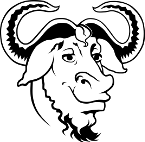
\includegraphics[width=0.4\textwidth]{figure/gnu_make.png}
            \caption{Logo GNU Operating System}
        \end{figure}

    \subsection{Docker}\label{docker}
    Docker è un progetto open-source sviluppato da Docker, Inc. disponibile dal 2013.
    Docker automatizza il rilascio e l'esecuzione di applicazioni all'interno di contenitori
    software. Fornisce quindi un astrazione aggiuntiva grazie alla virtualizzazione a
    livello di sistema operativo. Docker infatti utilizza le funzionalità di isolamento del
    kernel linux per consentire ai container di esistere in maniera indipendente l'uno dall'altro.
    Docker risulta molto utile anche per risparmiare spazio fisico sia sulla memoria principale
    in fase di esecuzione dei container, sia sulla memoria secondaria in termini di dimensione di
    immagini virtuali. Utilizzando i namespace del kernel linux si raggiunge l'isolamento tra container
    mentre con \textit{cgroup} si ottiene l'isolamento in termini di risorse del calcolatore.
    Nella figura \ref*{docker-scheme} è possibile visualizzare le differenze tra le comuni macchine
    virtuali e i container di Docker.
    \begin{figure}[H]\label{docker-scheme}
        \centering
        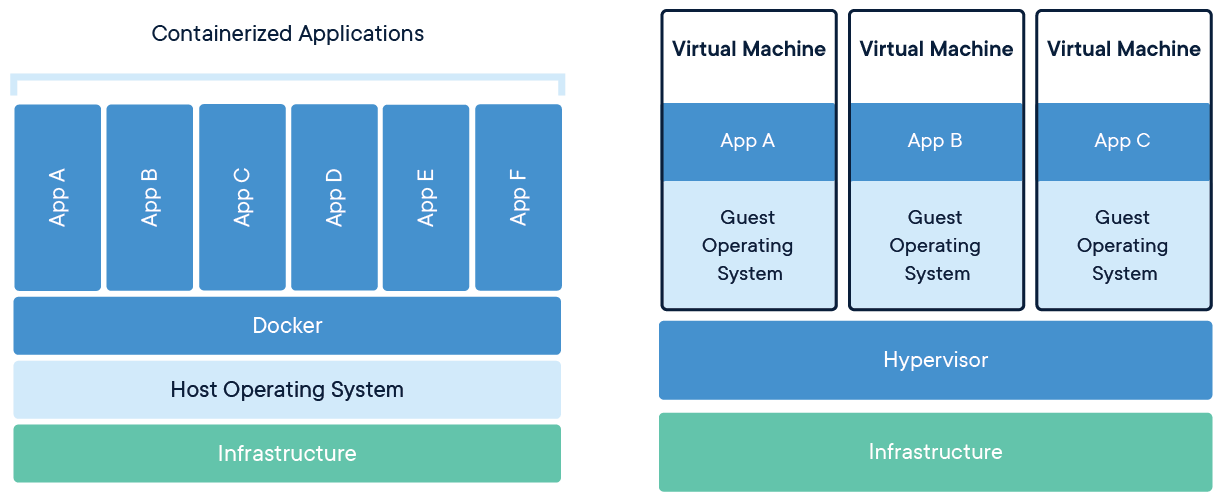
\includegraphics[width=\linewidth]{figure/docker-scheme.png}
        \caption{Differenze fra macchine virtuali e container Docker}
    \end{figure}
    Docker svolge il proprio compito grazie a più componenti che cooperano fra loro (\ref*{docker-components}).
    Il \textit{Docker Engine} è un applicazione client-server composto da:
    \begin{itemize}
        \item Servizio di tipo \textit{daemon} (servizio a lunga durata) composto da un server.
        \item API REST con la quale si può comunicare per gestire il daemon citato sopra.
        \item Interfaccia a linea di comando (invocabile tramite il comando \textit{docker})
    \end{itemize}

    Docker inoltre offre anche un servizio di salvataggio e gestione per le immagini dei container,
    \textit{Docker Hub}, dando la possibilità agli utenti di versionare i vari rilasci delle immagini
    che creano.
    \begin{figure}[H]\label{docker-components}
        \centering
        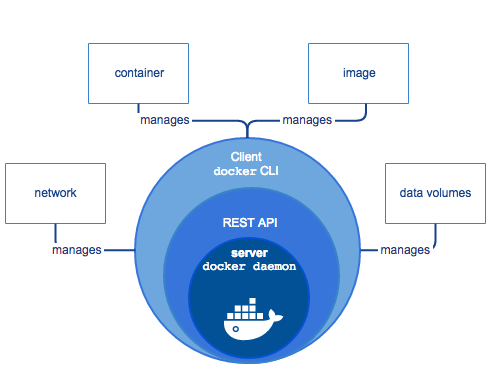
\includegraphics[width=\linewidth]{figure/engine-components-flow.png}
        \caption{Differenze fra macchine virtuali e container Docker}
    \end{figure}
    In questo progetto Docker è stato usato principalmente in congiunzione con Clion \ref*{clion}
    per utilizzare immagini ufficiali di Deal.II (\ref*{dealii}) e risolvere le dipendenze tra i vari componenti
    della libreria. Sono infatti presenti varie immagini per container di Deal.II
    al cui interno sono già soddisfatti i vincoli imposti dalle librerie usate (OpenMPI, Tbb, ecc).
    Docker rende quindi pressoché impossibili problemi di compatibilità di programmi tra diverse piattaforme e sistemi. 
    \begin{figure}[H]
        \centering
        
\includegraphics[width=\linewidth]{figure/docker.png}
        \caption{Logo Docker}
    \end{figure}


\section{Strumenti di visualizzazione e meshing}\label{visualizzazione}
Uno degli aspetti fondamentali quando si realizzano delle simulazioni CFD è la corretta costruzione e interpretazione della mesh (\ref*{mesh}) su cui operare.
Sarebbe impensabile costruire manualmente le mesh necessarie per simulare complessi condotti o ugelli, per questo motivo ci affidiamo a strumenti di meshing creati appositamente
per semplificare questo processo.

Le simulazioni di questo tipo, inoltre, generano una grande quantità di dati che possono risultare complicati da interpretare.
Nel caso di una simulazione di particelle infatti per ogni punto vengono salvate informazione riguardo
la posizione (un dato per ogni asse geometrico presente), la velocità (sempre per ogni asse geometrico) e temperatura per esempio.
Questi dati vengono salvati per ogni particella e per ogni intervallo di tempo discretizzato (time-step), si intuisce quindi
che la mole di dati con cui si ha a che fare in questi casi è importante.
Spesso inoltre questi dati vengono rappresentati secondo diversi formati, è quindi importante utilizzare un software di visualizzazione
capace di interpretare questi dati e mostrarli in maniera intuitiva.

    \subsection{Paraview}\label{paraview}
    Paraview è un applicazione open-source, multi-piattaforma di analisi e visualizzazione dati. Permette di creare
    visualizzazioni 2D o 3D in modo interattivo o programmatico, grazie alle sue funzionalità di processamento
    batch. Paraview può anche essere dispiegato in cluster di calcolatori per analizzare quantità di dati nell'ordine dei
    Peta-Byte. Paraview ormai è considerato uno standard nel mondo scientifico ed è usato in molti contesti differenti,
    sia a livello universitario che industriale.
    All'interno di questo progetto, Paraview è stato usato massivamente per tracciare il movimento delle particelle e soprattutto
    per verificare le condizioni di rimbalzo.

        \subsubsection{Paraview e OSPRay}\label{raytracing}
        Di recente Paraview ha aggiunto il supporto alla libreria di ray tracing sviluppata da Intel OSPRay \cite{WaldI2017O-AC}, che permette
        di realizzare dei render grafici sfruttando le tecniche di geometria ottica basate sul calcolo dei percorsi fatti dai fotoni stessi e
        dell'interazione fra essi e materiali realistici rispetto al punto di vista di una telecamera.
        
        \begin{figure}[H]
            \centering
            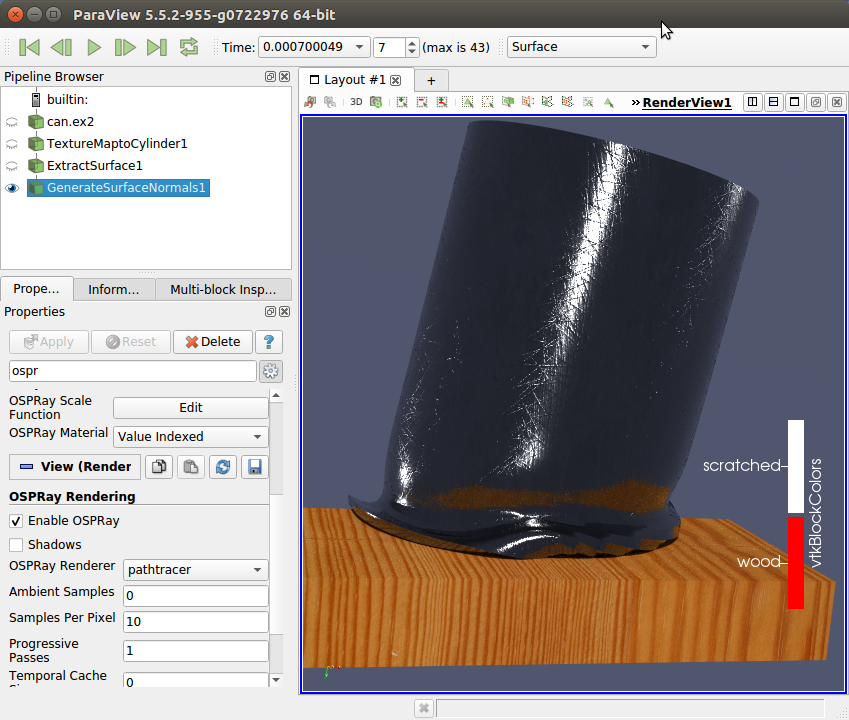
\includegraphics[width=\linewidth]{figure/ospray.png}
            \caption{Deformazione renderizzata con OSPRay in Paraview}
        \end{figure}
        
        \begin{figure}[H]
            \centering
            
\includegraphics[width=\linewidth]{figure/paraview.png}
            \caption{Logo Paraview}
        \end{figure}
        
        \subsection{SALOME}\label{salome}
        SALOME è una suite di strumenti open-source che fornisce moduli di pre e post processing per simulazioni, meshing e calcoli numerici su modelli.
        SALOME offre una serie di componenti che facilitano la creazione, modifica, importazione e esportazione di modelli CAD, generando per questi ultimi mesh in svariati formati
        comprensibili da altrettanti strumenti di CFD (compreso dealii \ref{dealii}). Un punto di forza di SALOME è la disponibilità di un interfaccia intuitiva che rende il processo
        di meshing molto più semplice e veloce. Durante lo svolgimento di questa tesi SALOME è stato utilizzato per generare la mesh finale dell'ugello responsabile per il deposito di materiale.

        \begin{figure}[H]
            \centering
            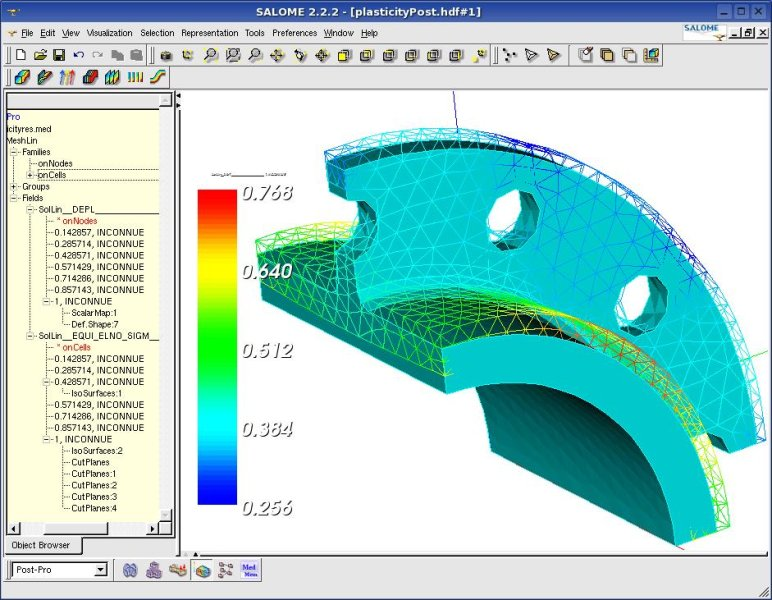
\includegraphics[width=\linewidth]{figure/salome.jpg}
            \caption{Interfaccia SALOME}
        \end{figure}
